\section{Background}\label{sc:background}
In this section, we provide a formalization of FMI co-simulation and a brief background on INTO-CPS Maestro 2.

\subsection{FMU Definitions}
To describe the formalization of FMUs, we adopt the vocabulary from \cite{gomes_lucio_vangheluwe_2019}. The main definitions of relevance to this paper will be presented, but readers are referred to the original publications for more information. This paper is only concerned with the initialization-phase of a co-simulation, making time of an FMU irrelevant. The formalization from Gomes et al.\cite{gomes_lucio_vangheluwe_2019} is extended with new definitions regarding algebraic loops, and convergence of fixed point iteration.
\begin{definition}[FMU]\label{def:fmu}
  An FMU with identifier $c$ is represented by the tuple   
  $$\tuple{\stateset{c}, \inputs{c}, \outputs{c}, \fset{c}, \fget{c}},$$
  where:
  \begin{inparadesc}
    \item $\stateset{c}$ represents the state space of FMU c;
    \item $\inputs{c}$ and $\outputs{c}$ the set of input and output variables, respectively;
    \item $\fset{c} : \stateset{c} \times \inputs{c} \times \values \to \stateset{c}$ and $\fget{c}: \stateset{c} \times \outputs{c} \to \values$ are functions to set the inputs and get the outputs, respectively (we abstract the set of values that each input/output variable can take as $\values$).
  \end{inparadesc}
\end{definition}

\begin{definition}[Scenario]\label{def:cosim_scenario}
  A scenario is a structure $\tuple{\fmus, \coupling}$ where each identifier $c \in \fmus$ is associated with an FMU, as defined in \cref{def:fmu}, and $\coupling(u)=y$ means that the output $y$ is connected to input $u$.
  Let $\allinputs = \bigcup_{c \in \fmus} \inputs{c}$ and $\alloutputs = \bigcup_{c \in \fmus} \outputs{c}$, then $\coupling : \allinputs \to \alloutputs$.
\end{definition}
Note a single output can connect to multiple inputs, but a single input can only rely on a single output.
The following definitions correspond to the operations that are permitted in the initialization phase of a co-simulation.

\begin{definition}[Output Computation]\label{def:getout}
The $\fget{c}(\dontcare, \outputvar{c})$ represents the calculation of output $\outputvar{c}$ of $c \in \fmus$. Given a co-simulation state, it checks whether all inputs that feed-through to $\outputvar{c}$ are defined.
\end{definition}

\begin{definition}[Input Computation]\label{def:setin}
The $\fset{c}(\dontcare, \inputvar{c}, \inputV)$ represents the setting of input $\inputvar{c}$  of $c \in \fmus$. Given a co-simulation state, it checks whether all outputs connected to $\inputvar{c}$ are defined.
\end{definition}

\begin{definition}[Fixed Point]\label{def:fixedpoint}
The $\fixedpoint{l}$ represents an ordered sequence of the setting or getting of all variables of a given SCC $l$, see \cref{def:loop} for a definition of SCC.
The $\fixedpoint{l} \subseteq \bigcup_{c \in \fmus} \set{\fget{c},\fset{c}}$ 
\end{definition}


\begin{definition}[Initialization]\label{def:initialization}
  Given a scenario $\tuple{\fmus, \coupling}$, we define the initialization procedure $\sequence{\initcall_i}_{i \in \setnat}$ as is a finite ordered sequence of FMU function calls that needs to be performed in the initialization of a co-simulation scenario. The ordered sequence is defined as: $\sequence{\functioncall_i}_{i \in \setnat} = \functioncall_0, \functioncall_1, \ldots$ with
  $\functioncall_i \in \initcall_{} = \bigcup_{l \in loops} \fixedpoint{l},$
  and $i$ denoting the order of the function call.
  Loops is defined as the set of all SCC see \cref{def:loop}.
\end{definition}

It should be noted that a trivial SCC (see \cref{def:loop}) is only a single get or set action and is not regarded as a fixed point outside \cref{def:initialization}, but just a simple computation.

\begin{definition}[Feed-through]\label{def:feedthrough}
  The input $\inputvar{c} \in \inputs{c}$ feeds through to output $\outputvar{c} \in \outputs{c}$, that is, $(\inputvar{c},\outputvar{c}) \in \feedthrough{c}$, when there exists $v_1, v_2 \in \values$ and $\state{c} \in \stateset{c}$, such that
  $
  \fget{c} (\fset{c}(\state{c}, \inputvar{c}, v_1), \outputvar{c}) \neq \fget{c} (\fset{c}(\state{c}, \inputvar{c}, v_2), \outputvar{c}).
  $
\end{definition}

%\claudio{I think the above two definitions should come before the initialization definition, as the later uses the former (I prefer a bottom up approach.). You can also, at the beginning of section 2.1, explain that you're going to ultimately define what the initialization procedure and algebraic loops are, but to do that, you have to define a couple of small things first. This allows the reader to understand why you define these small operations before getting to the bigger definitions.}

%\begin{definition}[Interconnected variable]
%An interconnected variable v of a co-simulation scenario $\tuple{\fmus, \coupling}$ is defined as $v \in \allinputs \cup \alloutputs$, then $\coupling : \allinputs \to \alloutputs$.
%The set all all interconnected variables is denoted: $V = \allinputs \cup \alloutputs$,
%\end{definition}

A graph of the dependencies of a co-simulation scenario is established from the interconnected variables by \cref{def:initialization_graph}. The graph is the foundation for the calculation of the initialization procedure and is therefore referred to as the Initialization Graph. The graph construction is similar to the one in \cite{Gomes2020b}, except the later focuses on a general co-simulation step, while this work focus on the initialization phase.

\begin{definition}[Initialization Graph]\label{def:initialization_graph}
  Given a co-simulation scenario $\tuple{\fmus, \coupling}$, and a set of feed-through dependencies $\bigcup_{c \in \fmus} \set{\feedthrough{c}}$, we define the Initialization Graph where each node represents a port $\outputvar{c} \in \outputs{c}$ or $\inputvar{c} \in \inputs{c}$ of some fmu $c \in \fmus$. The edges are created according to the following rules:
  \begin{compactenum}
    \item For each $c \in \fmus$ and $\inputvar{c} \in \inputs{c}$, if $\coupling(\inputvar{c}) = \outputvar{d}$, add an edge $\outputvar{d} -> \inputvar{c}$ (output to input).
    \item For each $c \in \fmus$ and $(\inputvar{c},\outputvar{c}) \in \feedthrough{c}$, add an edge $\inputvar{c} -> \outputvar{c}$ (input to output).
  \end{compactenum}
\end{definition}

The interconnections of FMU variables can lead to circular dependencies between the variables. An example of this behavior is the car suspension system that is presented in \cref{sec:case_study}. \cref{fig:fmu_cycle} shows the co-simulation scenario of the example and the Initialization Graph of the system. The Initialization Graph in \cref{fig:fmu_cycle} is annotated with the strongly connected components of the graph.

\begin{figure}
    \centering
    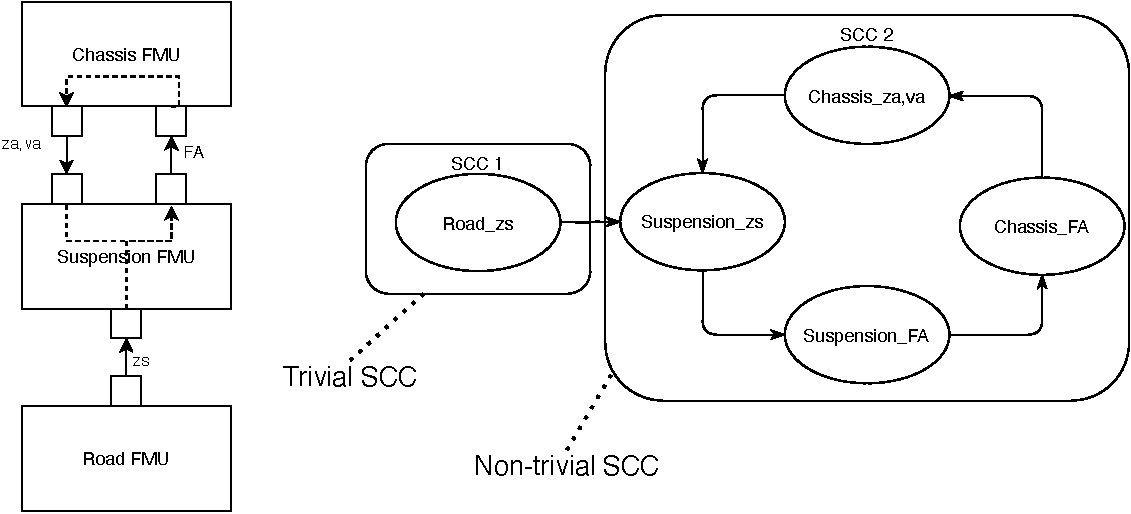
\includegraphics[width=1\textwidth]{images/quarter_car_SCC.pdf}
    \caption{An FMU co-simulation scenario of the Quarter car and its Initialization Graph denoted with SCCs.}
    \label{fig:fmu_cycle}
\end{figure}

The following definitions formalize the concept of an algebraic loop in a co-simulation scenario and define the problem these algebraic loops are introducing.
The definition of strongly connected components is adapted from the semantics of Causal Block Diagrams (see \cite{Gomes2020} for an overview).

\begin{definition}[Algebraic loops] \label{def:loop}
An algebraic loop is defined as a non-trivial, strongly connected component of the graph in \cref{def:initialization_graph}.
Formally, a strong connected component satisfies $\set{a,b \in SCC: \mathit{Path}(a,b)}$, where $\mathit{Path}(a,b)$ is true when there's a path (including an empty path from a node to itself) between nodes $a$ and $b$ ($\mathit{Path}(a,a)$ is always true).
An $SCC$ is non-trivial when it has more than one node.
\end{definition}

Since the edges of the graph represent dependencies between the variables, the value of every variable in a non-trivial strong component depends on itself.
Let $X$ denote a vector of one or more variables whose value depends on itself. The non-trivial strong component forms an equation with the form $F(X, U) = X$, where $F$ denotes the relations between the variables in the loop and $U$ denotes the variables whose values are calculated elsewhere. 
This means that algebraic loops need to be handled using fixed point iterations\cite{Gomes2018}. 

An example of a co-simulation scenario where fixed point iteration is needed can be seen in \cref{fig:fmu_cycle} where the Initialization Graph of the quarter car system from \cref{sec:case_study} is shown.

% The initialization of the system requires the application of fixed point iteration, as defined \cref{def:fixedpoint}.
%\begin{definition}[Fixed point iteration of an Initialization procedure]\label{def:fixedpoint}
%A fixed point iteration of given loop $l$ consist of the order sequence of functions calls:
%$\forall v \in l: \exists op \in \fixedpoint{l} : op = \fget{}(\dontcare, v) \lor op = \fset{}(\dontcare, v, \dontcare)$.
%Performing a iteration on a co-simulation state leads to a new state to $\fixedpoint{l}(\state{n}) = \state{n + 1}$
%The fixed point iteration is performed in order to find a convergent initialization state as defined in \cref{def:convergence}.
%\end{definition}

%\claudio{The above defintions is strange. If there's an algebraic loop, you cannot have an initialization procedure. At least not the way it is currently defined. Also I feel that you don't really need to define the fixed point iteration. We just need to reformulate the initialization procedure so that it matches what your plugin should output.}

A fixed point iteration technique is not guaranteed to convergence if the system is unstable. The fixed point is as a numerical fixed point that approximates a limit if such a value exist (the system is stable). It means that an upper bound of the number of repetitions needs to be established to ensure termination. In the case of a non-converging algebraic loop, the simulation should be stopped since the result of the co-simulation scenario would not be trustworthy. The criteria of a valid co-simulation scenario are specified in \cref{def:convergence}.

\begin{definition}[Convergence of Fixed point iteration]\label{def:convergence}
A fixed point iteration converges if a finite number of iterations will make the difference of the output value of the same operation between two following iterations within a certain threshold $\epsilon$.\\
Formally, 
$\exists n \in \setnat: |F(X^{n+1}, U) - F(X^{n}, U)| \leq \epsilon$.
\end{definition}

\subsection{INTO-CPS Maestro 2}
INTO-CPS Maestro 2\footnote{currently in alpha \url{https://github.com/INTO-CPS-Association/maestro/tree/2.0.0-alpha}.}~\cite{Thule2020a} is a framework for creating simulation specifications and executing such specifications. The framework is FMI-based and set to supersede Maestro~\cite{Maestro} with the main goal of supporting research into co-simulation based on FMI. 

The philosophy of the framework is to separate the specification of a co-simulation from the execution. This allows one to inspect and verify, manually or automatically, how a given co-simulation is to be executed. 

A specification is expressed in the domain-specific language called Maestro Base Language (MaBL), and it is explicit, such that the application of, i.e., FMUs are transparent. Expansion plugins can assist in creating such MaBL specifications, and one can apply expansion plugins that, in turn, generate the MaBL code. The plugin described in this paper is such an expansion plugin. The application of a plugin is evident in a MaBL specification. Upon processing of the specification, a new specification is created where the application of a plugin is replaced by the MaBL code generated by the plugin. This process is known as expansion, and a specification without any expansions remaining is a fully expanded MaBL specification. An example of a part of the folded MaBL specification of the case study example of \cref{sec:case_study} can be seen below.

\begin{lstlisting}[language=C++]
simulation
import Initializer;
{
FMI2 chassis = load("FMI2", "{8c4e810f-3df3-4a00-8276-176fa3c9f000}", "src/chassis-c.fmu");
...
IFmuComponent components[3]={chassis,suspension, road};
expand initialize(components,START_TIME, END_TIME);
...
}
\end{lstlisting}
To conduct a co-simulation, Maestro2 also features an interpreter that can execute a fully expanded MaBL specification, resulting in the execution of the co-simulation.